% Cube-in-Hand Calibration 발표자료 (1~11장)
%
% 컴파일: XeLaTeX 또는 LuaLaTeX 로 컴파일해야 한글이 나온다.
%   Overleaf: 왼쪽 위 Menu > Compiler > XeLaTeX 선택
%   로컬:     xelatex calibration_1_11.tex   (두 번 실행)
%
% 원문: CALIBRATION_EXPLANATION_LATEX.md 의 1장부터 11장까지
% 문체: 슬라이드는 개조식, 원문 문서는 구어체

\documentclass[aspectratio=169,11pt]{beamer}

\usepackage{kotex}
% 한글 글꼴: 나눔바른고딕 (Regular + Bold 보유). 발표 화면에서 읽기 좋다.
\setmainhangulfont{NanumBarunGothic}
\setsanshangulfont{NanumBarunGothic}
\setmonohangulfont{NanumGothicCoding}
\usepackage{amsmath}
\usepackage{amssymb}
\usepackage{booktabs}
\usepackage{array}
\usepackage{tabularx}
\usepackage{graphicx}

\usetheme{Madrid}
\usecolortheme{whale}
\setbeamertemplate{navigation symbols}{}
\setbeamertemplate{caption}[numbered]
\setbeamerfont{frametitle}{size=\large}
\setbeamerfont{block title}{size=\normalsize}

% ── 표지 레이아웃 직접 정의 ──────────────────────────────
\definecolor{titlegray}{HTML}{55606E}
\setbeamertemplate{title page}{%
  \vspace*{\fill}
  \begin{center}
    {\usebeamercolor[fg]{structure}\fontsize{31}{36}\selectfont
     \textbf{\inserttitle}\par}
    \vspace{4mm}
    {\usebeamercolor[fg]{structure}\rule{0.40\textwidth}{1.2pt}\par}
    \vspace{4mm}
    {\color{titlegray}\fontsize{13}{18}\selectfont \insertsubtitle\par}
    \vspace{13mm}
    {\color{titlegray!60}\rule{0.12\textwidth}{0.5pt}\par}
    \vspace{4mm}
    {\color{titlegray}\fontsize{13}{17}\selectfont \insertauthor\par}
    \ifx\insertinstitute\empty\else
      \vspace{2mm}{\color{titlegray}\small\insertinstitute\par}
    \fi
  \end{center}
  \vspace*{\fill}
}

% ── 11장 Corrected-FK 수록 여부 ──────────────────────────
% 아직 검증이 끝나지 않은 방식이라 현재 발표본에서는 제외한다.
% 되살리려면 아래 한 줄을 \correctedfktrue 로 바꾸기만 하면 된다.
% (11장 본문과 1.4 / 5 / 9장의 관련 서술이 함께 되돌아온다)
\newif\ifcorrectedfk
\correctedfkfalse

% 표 안에서 줄 간격을 조금 넓힌다
\renewcommand{\arraystretch}{1.3}

% ── 변환행렬 표기 ────────────────────────────────────────
% 축약 기호(C_i, X, Z, G, F, V, A ...)를 쓰지 않고
% 항상 <도착>T<출발> 형태로 적는다. 곱셈에서 중간 좌표계가
% 맞물려 사라지는 것이 눈에 보이게 하기 위함.
% \T{도착}{출발}  또는  \T[윗표시]{도착}{출발}
\newcommand{\T}[3][]{{}^{#2}\mathbf{T}^{#1}_{#3}}   % 예: \T{B}{C_i}, \T[(0)]{B}{C_i}
\newcommand{\Tb}[2]{{}^{#1}\overline{\mathbf{T}}_{#2}} % 세트 공통(평균) 변환
\newcommand{\Th}[3][]{{}^{#2}\widehat{\mathbf{T}}^{#1}_{#3}} % 최적화로 찾은 추정값
% 큐브 좌표계의 여러 추정치 = 서로 다른 좌표계 이름으로 구분
\newcommand{\Oref}{O^{\mathrm{ref}}}   % 목적함수가 맞추는 기준 자세
\newcommand{\Ofk}{O^{\mathrm{fk}}}     % raw FK가 말하는 큐브
\newcommand{\Ovis}{O^{\mathrm{vis}}}   % vision 합의가 말하는 큐브
\newcommand{\Ocorr}{O^{\mathrm{corr}}} % 공통 보정 후의 FK 큐브
\newcommand{\Oanc}{O^{\mathrm{anc}}}   % gate를 거쳐 확정된 anchor

\title[Cube-in-Hand Calibration]{Cube-in-Hand Calibration}
\subtitle{마커 큐브와 로봇 FK를 함께 쓰는 멀티카메라 캘리브레이션}
\author{이수민, 김지우}
\institute{}
\date{}

\begin{document}

\begin{frame}
  \titlepage
\end{frame}

\begin{frame}{다루는 내용}
  \tableofcontents
\end{frame}

%==================================================================
\section{1. 캘리브레이션이란, 그리고 카메라 구성}
%==================================================================

\begin{frame}{1.1 로봇과 카메라는 서로 다른 것을 안다}
  \begin{columns}[T]
    \begin{column}{0.48\textwidth}
      \begin{block}{로봇이 아는 것}
        \begin{minipage}[t][26mm][t]{\linewidth}
          \begin{itemize}
            \item 관절 각도 $\rightarrow$ \textbf{자기 손끝 위치} 계산 가능
            \item 주변에 무엇이 어디 있는지는 모름
          \end{itemize}
        \end{minipage}
      \end{block}
    \end{column}
    \begin{column}{0.48\textwidth}
      \begin{block}{카메라가 아는 것}
        \begin{minipage}[t][26mm][t]{\linewidth}
          \begin{itemize}
            \item \textbf{물체의 위치}를 볼 수 있음
            \item 단, 자기 렌즈 앞을 기준으로만 말함
            \item ``내 앞 $60\,\mathrm{cm}$, 오른쪽 $10\,\mathrm{cm}$''
          \end{itemize}
        \end{minipage}
      \end{block}
    \end{column}
  \end{columns}
  \vfill
  \begin{alertblock}{캘리브레이션이란?}
    둘 사이의 번역기를 만드는 일\\
    카메라가 말한 위치 $\rightarrow$ 로봇이 움직일 수 있는 좌표
  \end{alertblock}
\end{frame}

\begin{frame}{1.2 왜 중요한가}
  \begin{itemize}
    \item 인식이 정확해도 번역기가 틀어지면 로봇은 엉뚱한 곳으로 감
  \end{itemize}
  \vfill
  \begin{block}{예시}
    \begin{itemize}
      \item 카메라의 물체 인식 오차: $1\,\mathrm{mm}$
      \item 카메라와 로봇 사이 관계의 오차: $10\,\mathrm{mm}$
      \item $\Rightarrow$ 로봇이 실제 가는 곳은 $10\,\mathrm{mm}$ 빗나감
      \item $\Rightarrow$ 인식 성능을 올려도 이 오차는 그대로
    \end{itemize}
  \end{block}
  \vfill
  \begin{alertblock}{}
    캘리브레이션 정확도 = 전체 시스템 정확도의 \textbf{상한}
  \end{alertblock}
\end{frame}

\begin{frame}{1.3 카메라가 여러 대면 문제가 하나 더}
  카메라마다 자기 자신을 원점으로 사용
  \begin{itemize}
    \item 카메라 $0$: 큐브가 자기 \textbf{앞}에 있다
    \item 카메라 $1$: 같은 큐브가 자기 \textbf{오른쪽}에 있다
    \item 그리퍼 카메라: 같은 큐브가 자기 \textbf{아래}에 있다
  \end{itemize}
  \vfill
  세 답은 모순이 아님. 기준 좌표계가 다를 뿐
  \vfill
  \begin{block}{해야 할 일}
    모든 관측을 공통 기준인 로봇 베이스 좌표계 $B$로 옮기기\\
    $\rightarrow$ 여러 카메라가 같은 물체에 같은 좌표를 말하게 됨
  \end{block}
\end{frame}

\begin{frame}{1.4 구성 1: eye-in-hand (카메라가 손에 붙음)}
  카메라를 로봇 손목에 장착 $\rightarrow$ 로봇이 움직이면 카메라도 함께 움직임
  \vfill
  \begin{block}{물체를 보는 경로}
    \centering
    베이스 $\rightarrow$ 손 $\rightarrow$ 카메라 $\rightarrow$ 물체
  \end{block}
  \vfill
  \begin{columns}[T]
    \begin{column}{0.48\textwidth}
      \begin{block}{찾아야 하는 것}
        \begin{minipage}[t][20mm][t]{\linewidth}
          \begin{itemize}
            \item \textbf{손과 카메라 사이 관계} 하나
            \item 나사로 고정 $\rightarrow$ 안 변함
          \end{itemize}
        \end{minipage}
      \end{block}
    \end{column}
    \begin{column}{0.48\textwidth}
      \begin{block}{어떻게 푸는가}
        \begin{minipage}[t][20mm][t]{\linewidth}
          \begin{itemize}
            \item 로봇을 여러 자세로 옮기며 같은 물체를 촬영
            \item 손 위치는 로봇이 알려줌
          \end{itemize}
        \end{minipage}
      \end{block}
    \end{column}
  \end{columns}
  \vfill
  \centering
  물체에 가까이 다가가 볼 수 있어 정밀함. 대신 한 번에 보이는 범위가 좁음
\end{frame}

\begin{frame}{1.5 구성 2: eye-to-hand (카메라가 밖에 고정)}
  카메라를 작업대에 고정 $\rightarrow$ 로봇이 움직여도 카메라는 그대로
  \vfill
  \begin{block}{물체를 보는 경로}
    \centering
    베이스 $\rightarrow$ 카메라 $\rightarrow$ 물체
    \qquad {\small(손을 거치지 않음. 한 칸 짧다)}
  \end{block}
  \vfill
  \begin{columns}[T]
    \begin{column}{0.48\textwidth}
      \begin{block}{찾아야 하는 것}
        \begin{minipage}[t][20mm][t]{\linewidth}
          \begin{itemize}
            \item \textbf{베이스와 카메라 사이 관계} 하나
          \end{itemize}
        \end{minipage}
      \end{block}
    \end{column}
    \begin{column}{0.48\textwidth}
      \begin{block}{어떻게 푸는가}
        \begin{minipage}[t][20mm][t]{\linewidth}
          \begin{itemize}
            \item 로봇 손에 마커를 붙이고 여러 자세로 움직임
            \item 같은 마커를 로봇은 계산으로, 카메라는 사진으로 파악
              $\rightarrow$ 두 값을 맞춤
          \end{itemize}
        \end{minipage}
      \end{block}
    \end{column}
  \end{columns}
  \vfill
  \centering
  작업 공간 전체를 한눈에 봄. 대신 거리가 멀어 정밀도가 낮고, 로봇 팔에 가려지기도 함
\end{frame}

\begin{frame}{1.6 구성 3: eye-to-hand 여러 대}
  가림과 사각지대를 줄이려고 고정 카메라를 여러 대 설치
  \vfill
  \begin{alertblock}{카메라를 한 대씩 따로 캘리브레이션하면}
    각 카메라는 나름대로 맞게 나오지만 \textbf{서로 조금씩 어긋남}\\
    $\rightarrow$ 같은 물체를 두고 \textbf{서로 다른 좌표}를 말하게 됨 (1.3절)
  \end{alertblock}
  \vfill
  \begin{block}{그래서 필요한 것}
    \begin{itemize}
      \item 모든 카메라가 \textbf{같은 물체를 동시에} 보게 함
      \item 모두가 같은 답을 말하도록 카메라 위치를 \textbf{한꺼번에} 조정
      \item 이때 새로 생기는 미지수: \textbf{그때 물체가 어디 있었는가}
    \end{itemize}
  \end{block}
  \vfill
  \centering
  {\small 한 대씩 맞추면 어긋난 채로 남음 $\rightarrow$ 전부 함께 맞춰야 함}
\end{frame}

\begin{frame}{1.7 구성 4: 여기에 eye-in-hand까지 추가}
  고정 카메라 여러 대 \textbf{+} 손목 카메라 하나 = 이 프로젝트의 구성
  \vfill
  \begin{block}{왜 손목 카메라를 더하는가}
    \begin{itemize}
      \item 로봇과 함께 움직이며 \textbf{여러 각도에서} 같은 물체를 봄
      \item 고정 카메라 A와 B가 겹쳐 보는 곳이 없어도,
        손목 카메라는 A 앞에서도 찍고 B 앞에서도 찍음\\
        $\rightarrow$ \textbf{두 카메라를 잇는 연결 고리}가 됨
      \item 물체에 가까이 가서 찍으므로 \textbf{더 정밀한 관측}이 추가됨
    \end{itemize}
  \end{block}
  \vfill
  \begin{alertblock}{이제 한 번에 찾아야 하는 것}
    고정 카메라들의 자세 (여러 개) \ $+$ \ 손-카메라 관계 (한 개)
    \ $+$ \ 물체 자세 (촬영 상황마다)
  \end{alertblock}
  \vfill
  \centering
  {\small 5장에서 기호로, 6장에서 식으로 다시 정리}
\end{frame}

\begin{frame}{1.8 이 프로젝트의 설정}
  \begin{itemize}
    \item 로봇 그리퍼가 큐브를 잡고 여러 위치로 옮김
    \item 큐브를 한 번 놓은 상태 = \textbf{세트}
  \end{itemize}
  \vfill
  \begin{block}{카메라 두 종류}
    \begin{itemize}
      \item \textbf{고정 카메라}: 작업 공간 주변에 고정. 여러 대
      \item \textbf{그리퍼 카메라}: 로봇 손목에 부착. 로봇과 함께 이동
    \end{itemize}
  \end{block}
  \vfill
  \begin{alertblock}{9\,--\,\ifcorrectedfk 11\else 10\fi 장의 핵심 주제}
    로봇이 큐브를 잡고 있음 $\rightarrow$ 관절값으로 큐브 위치를 짐작 가능\\
    이 정보를 \textbf{얼마나 믿을 것인가}
  \end{alertblock}
\end{frame}

\begin{frame}{1.9 전체 시스템 구성과 그림 표기}
  \centering
  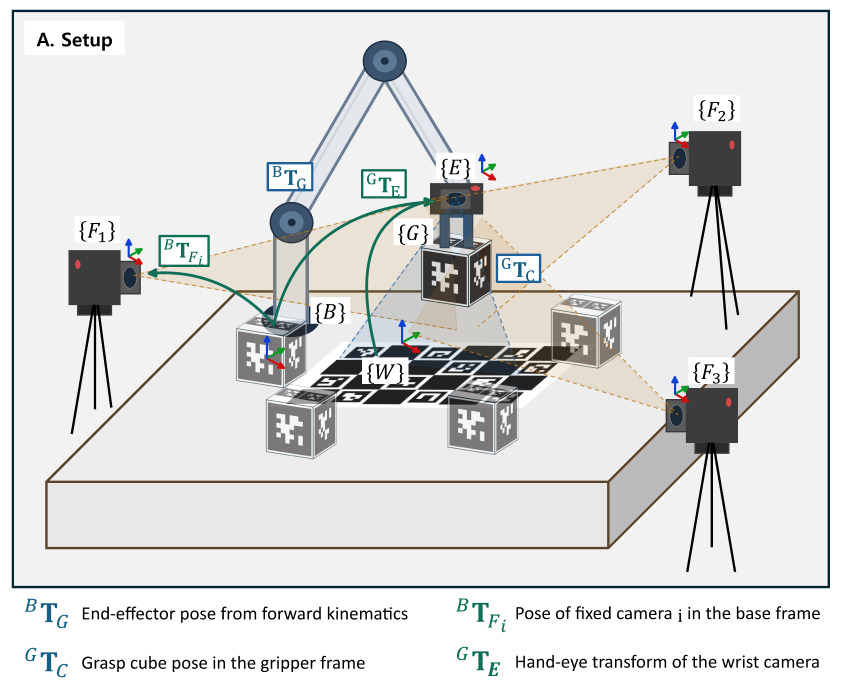
\includegraphics[
    height=0.64\textheight,
    trim=0 106bp 0 0,
    clip
  ]{cube_in_hand_calibration_setup.png}

  \vspace{1mm}
  {\scriptsize
    그림의 $F_i,\,E,\,C$는 본문에서 각각 $C_i,\,C_g,\,O$로 표기한다.\par
    그림의 $\T{B}{G}$는 본문의 $\T{B}{G,e}$에 해당하며,
    $\T{G}{C}$는 그리퍼--파지 큐브 사이의 고정 관계이다.\par
    $W$는 보드 좌표계이며, 이후 캘리브레이션 식에는 사용하지 않는다.
  }
\end{frame}

%==================================================================
\section{2. 좌표계 기호}
%==================================================================

\begin{frame}{2. 먼저 좌표계 기호를 정리}
  \begin{center}
    \begin{tabular}{cl}
      \toprule
      기호 & 의미 \\
      \midrule
      $B$      & 로봇 베이스 좌표계 \\
      $C_i$    & $i$번째 고정 카메라 좌표계 \\
      $G$      & 로봇 그리퍼 좌표계 \\
      $C_g$    & 그리퍼에 부착된 카메라 좌표계 \\
      $O$      & 큐브 또는 캘리브레이션 물체 좌표계 \\
      $s$      & 큐브를 놓은 세트 번호 \\
      $e$      & 그리퍼 카메라 촬영 이벤트 번호 \\
      $s(e)$   & 이벤트 $e$가 속한 세트 번호 \\
      \bottomrule
    \end{tabular}
  \end{center}
\end{frame}

\begin{frame}{2. 변환 표기를 읽는 법}
  \[
    {}^{A}\mathbf{T}_{B}
  \]
  \begin{block}{읽는 법}
    좌표계 $B$에서 표현된 값 $\rightarrow$ 좌표계 $A$에서 표현하도록 바꾸는 변환
  \end{block}
  \vfill
  \begin{itemize}
    \item 위 첨자 $A$ = \textbf{도착} 좌표계
    \item 아래 첨자 $B$ = \textbf{출발} 좌표계
  \end{itemize}
\end{frame}

%==================================================================
\section{3. 변환행렬}
%==================================================================

\begin{frame}{3. 변환행렬은 무엇인가}
  강체 자세 = 회전 + 이동 $\rightarrow$ $4 \times 4$ 동차변환행렬
  \[
    \mathbf{T}
    =
    \begin{bmatrix}
      \mathbf{R} & \mathbf{t} \\
      \mathbf{0}^{\mathsf T} & 1
    \end{bmatrix},
    \qquad
    \mathbf{R}\in\mathrm{SO}(3),
    \qquad
    \mathbf{t}\in\mathbb{R}^{3}
  \]
  \begin{itemize}
    \item $\mathbf{R}$: 물체가 어느 방향을 보는지. $3 \times 3$ 회전행렬
    \item $\mathbf{t}$: 물체가 어디에 있는지. $3 \times 1$ 이동벡터
  \end{itemize}
  \vfill
  좌표점 $\mathbf{p}_B$를 좌표계 $A$로 옮기기
  \[
    \begin{bmatrix} \mathbf{p}_A \\ 1 \end{bmatrix}
    =
    {}^{A}\mathbf{T}_{B}
    \begin{bmatrix} \mathbf{p}_B \\ 1 \end{bmatrix}
  \]
\end{frame}

\begin{frame}{3. 이 형식을 쓰는 이유}
  \begin{enumerate}
    \item \textbf{위치와 방향을 한 값으로 묶음}
      \begin{itemize}
        \item 따로 관리하면 계산할 때마다 둘을 맞춰야 함
        \item 묶으면 자세 전체가 변수 하나
      \end{itemize}
      \vspace{2mm}
    \item \textbf{좌표계 갈아타기를 곱셈 한 번으로}
      \begin{itemize}
        \item 회전만이면 $3 \times 3$으로 충분
        \item 이동은 곱셈이 아니라 덧셈 $\rightarrow$ 그대로는 안 섞임
        \item 마지막 행에 $1$을 붙여 $4 \times 4$로 $\rightarrow$ 이동도 곱셈 안으로
        \item $\rightarrow$ 여러 좌표계를 거치는 경로를 행렬 곱만으로 연결 (3.1절)
      \end{itemize}
      \vspace{2mm}
    \item \textbf{되돌리기가 쉬움}
      \begin{itemize}
        \item 역행렬 하나로 방향을 반대로 (3.2절)
      \end{itemize}
  \end{enumerate}
\end{frame}

\begin{frame}{3.1 변환행렬을 곱한다는 뜻}
  경로를 차례대로 연결
  \[
    {}^{A}\mathbf{T}_{C}
    =
    {}^{A}\mathbf{T}_{B}\,
    {}^{B}\mathbf{T}_{C}
  \]
  \vfill
  행렬 내부까지 펼치면
  \[
    \begin{bmatrix}
      \mathbf{R}_1 & \mathbf{t}_1 \\
      \mathbf{0}^{\mathsf T} & 1
    \end{bmatrix}
    \begin{bmatrix}
      \mathbf{R}_2 & \mathbf{t}_2 \\
      \mathbf{0}^{\mathsf T} & 1
    \end{bmatrix}
    =
    \begin{bmatrix}
      \mathbf{R}_1\mathbf{R}_2 & \mathbf{R}_1\mathbf{t}_2+\mathbf{t}_1 \\
      \mathbf{0}^{\mathsf T} & 1
    \end{bmatrix}
  \]
\end{frame}

\begin{frame}{3.2 역행렬의 뜻}
  변환의 방향을 반대로
  \[
    \mathbf{T}^{-1}
    =
    \begin{bmatrix}
      \mathbf{R}^{\mathsf T} & -\mathbf{R}^{\mathsf T}\mathbf{t} \\
      \mathbf{0}^{\mathsf T} & 1
    \end{bmatrix}
  \]
  \begin{itemize}
    \item 회전은 전치행렬 $\mathbf{R}^{\mathsf T}$로 되돌림
    \item 이동도 그 회전 좌표계에 맞추어 반대로 적용
  \end{itemize}
  \vfill
  \begin{block}{역행렬을 쓰는 곳}
    \begin{enumerate}
      \item 아는 변환의 방향이 필요한 방향과 반대일 때
      \item 두 자세의 차이를 잴 때 (자세끼리는 뺄셈이 성립하지 않음, 7장)
      \item 곱해진 식에서 아는 항을 걷어내고 미지수만 남길 때 (이항과 같음)
    \end{enumerate}
  \end{block}
\end{frame}

%==================================================================
\section{4. 카메라가 측정하는 것}
%==================================================================

\begin{frame}{4. 카메라가 실제로 측정하는 것}
  \begin{itemize}
    \item 이미지에서 보드나 큐브의 코너를 검출
    \item \textbf{PnP}를 풀어서 자세를 얻음
  \end{itemize}
  \vfill
  PnP = Perspective-$n$-Point\\
  사진 한 장으로 물체가 카메라 기준 어디에 어떤 방향인지 알아내는 방법
  \vfill
  \begin{block}{PnP에 필요한 두 가지}
    \begin{enumerate}
      \item \textbf{물체 위 점들의 3차원 좌표} (물체 자신의 좌표계 기준)
        \begin{itemize}
          \item 한 변 $50\,\mathrm{mm}$ 체커보드 $\rightarrow$
            코너가 $(0,0,0)$, $(50,0,0)$, $(0,50,0)$
          \item 설계 도면에서 이미 아는 값
        \end{itemize}
      \item \textbf{같은 점들의 2차원 픽셀 좌표} (코너 검출 알고리즘이 제공)
    \end{enumerate}
  \end{block}
\end{frame}

\begin{frame}{4. PnP의 전제와 출력}
  \begin{itemize}
    \item 3차원 좌표와 픽셀 좌표의 짝을 여러 개 모으면 자세를 역으로 풀 수 있음
    \item 이름의 $n$ = 그 짝의 개수. 원리상 최소 $3$개, 실제로는 더 많이 사용
  \end{itemize}
  \vfill
  \begin{block}{전제: 카메라 내부파라미터를 미리 알아야 함}
    \begin{itemize}
      \item 초점거리, 이미지 중심 등
      \item 3차원 점이 이미지의 어느 픽셀에 맺히는지를 정하는 값
      \item 캘리브레이션 이전에 따로 구해 둠
    \end{itemize}
  \end{block}
  \vfill
  \begin{alertblock}{정리}
    PnP의 출력 = 관측값 $\mathbf{Z}$ = \textbf{카메라 좌표계에서 본} 물체의 자세
  \end{alertblock}
\end{frame}

\begin{frame}{4. 재투영오차: 얼마나 맞는지 재는 자}
  지금 알고 있는 값으로 \textbf{코너가 사진의 어디에 찍힐지 계산}하고,
  실제로 검출된 픽셀과 비교
  \[
    \mathbf{e}_j
    =
    \underbrace{
      \pi\!\left(\left(\T{B}{C}\right)^{-1}\T{B}{O},\ \mathbf{p}_j\right)
    }_{\text{계산한 픽셀}}
    \ -\
    \underbrace{\mathbf{u}_j}_{\text{검출된 픽셀}}
  \]
  \begin{itemize}
    \item $\mathbf{p}_j$: 물체 도면상의 $j$번째 코너 좌표
      \quad $\mathbf{u}_j$: 사진에서 찾은 그 코너의 픽셀
    \item $\pi$: 내부파라미터와 렌즈 왜곡을 써서 $3$차원 점을 픽셀로 옮기는 함수
    \item 단위는 \textbf{픽셀}. 코너 하나마다 값이 하나씩 나옴
  \end{itemize}
  \vfill
  \begin{block}{PnP도 사실 이것을 줄여서 자세를 찾는다}
    자세를 이리저리 바꿔보며 재투영오차가 가장 작아지는 자세를 고르는 것
  \end{block}
\end{frame}

\begin{frame}{4.1 -- 4.3 관측값의 정의}
  이미 측정이 끝나 \textbf{바꿀 수 없는} 값 세 가지
  \vfill
  \textbf{4.1 고정 카메라 관측} \hfill $\T{C_i}{O,s}$
  \vspace{-1mm}
  \begin{itemize}
    \item 세트 $s$의 큐브가 고정 카메라 $i$에서 어떻게 보였는가
  \end{itemize}
  \vfill
  \textbf{4.2 그리퍼 카메라 관측} \hfill $\T{C_g}{O,e}$
  \vspace{-1mm}
  \begin{itemize}
    \item 이벤트 $e$에서 큐브가 그리퍼 카메라에 어떻게 보였는가
  \end{itemize}
  \vfill
  \textbf{4.3 로봇 FK로 아는 그리퍼 자세} \hfill $\T{B}{G,e}$
  \vspace{-1mm}
  \begin{itemize}
    \item 촬영 순간 그리퍼의 위치와 방향. 관절각으로부터 FK로 계산
  \end{itemize}
  \vfill
  \begin{block}{}
    \centering
    앞의 둘은 \textbf{큐브 $O$에서 카메라로}, 마지막은
    \textbf{그리퍼 $G$에서 베이스 $B$로} 옮기는 변환\\
    $\rightarrow$ 출발ㆍ도착 좌표계가 달라 그대로는 이어붙일 수 없음 (6장에서 연결)
  \end{block}
\end{frame}

\begin{frame}{4.3 FK란}
  FK = Forward Kinematics = \textbf{순기구학}
  \vfill
  \begin{columns}[c]
    \begin{column}{0.46\textwidth}
      \begin{itemize}
        \item 입력: 각 관절이 몇 도 꺾여 있는지 + 링크 길이 등 설계값
        \item 출력: 손끝이 베이스 기준 어디에 어떤 방향으로 있는지
      \end{itemize}
      \vspace{4mm}
      \begin{block}{중요한 점}
        카메라 없이 \textbf{로봇 자신의 관절 센서만으로} 얻는 값
      \end{block}
    \end{column}
    \begin{column}{0.50\textwidth}
      \centering
      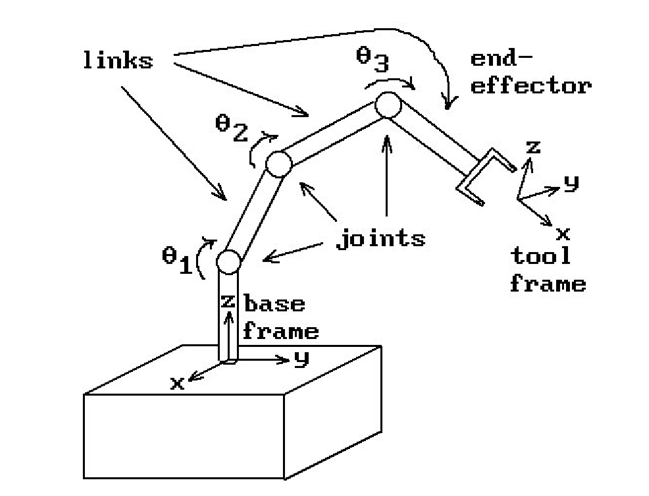
\includegraphics[width=\linewidth]{fk.png}
    \end{column}
  \end{columns}
\end{frame}

%==================================================================
\section{5. 찾아야 하는 미지수}
%==================================================================

\begin{frame}{5. 우리가 찾아야 하는 미지수}
  \textbf{5.1 고정 카메라 외부파라미터} \hfill $\T{B}{C_i}$
  \vspace{-1mm}
  \begin{itemize}
    \item 고정 카메라 $i$가 베이스 기준 어디에 어떻게 놓여 있는가
  \end{itemize}
  \vfill
  \textbf{5.2 그리퍼와 그리퍼 카메라 사이의 hand-eye 변환} \hfill $\T{G}{C_g}$
  \vspace{-1mm}
  \begin{itemize}
    \item 손목 카메라가 그리퍼에 어떻게 붙어 있는가. 세트와 무관하게 하나
  \end{itemize}
  \vfill
  \textbf{5.3 세트별 큐브 자세} \hfill $\T{B}{O,s}$
  \vspace{-1mm}
  \begin{itemize}
    \item 세트 $s$에서 큐브가 베이스 기준 실제로 어디에 있었는가
  \end{itemize}
  \vfill
  \begin{alertblock}{}
    \ifcorrectedfk
      세 FK 방식의 차이 = $\T{B}{O,s}$를 자유롭게 찾는가 / FK 값에 고정하는가 /
      보정된 anchor에 고정하는가
    \else
      두 FK 방식의 차이 = $\T{B}{O,s}$를 자유롭게 찾는가 / FK 값에 고정하는가
    \fi
  \end{alertblock}
\end{frame}

%==================================================================
\section{6. 두 종류 카메라의 관측 경로}
%==================================================================

\begin{frame}{6.1 고정 카메라 경로}
  베이스 $\rightarrow$ 고정 카메라 $\rightarrow$ 큐브
  \[
    \T{B}{C_i}\,
    \T{C_i}{O,s}
    =
    \T{B}{O,s}
  \]
  \begin{itemize}
    \item 가운데 $C_i$가 위아래로 맞물려 사라짐 $\rightarrow$ 경로가 이어짐 (3.1절)
    \item 왼쪽: 모르는 값 (5.1절) \quad 가운데: 카메라가 준 값 (4.1절)
  \end{itemize}
  \vfill
  \begin{block}{}
    \centering
    카메라 자세를 하나 가정하면 $\T{B}{C_i}\,\T{C_i}{O,s}$ 는\\
    ``$i$번 카메라 말로는 큐브가 여기 있다''는 \textbf{예측} 하나가 됨
  \end{block}
\end{frame}

\begin{frame}{6.2 그리퍼 카메라 경로}
  베이스 $\rightarrow$ 그리퍼 $\rightarrow$ 카메라 $\rightarrow$ 큐브
  \[
    \T{B}{G,e}\,
    \T{G}{C_g}\,
    \T{C_g}{O,e}
    =
    \T{B}{O,s(e)}
  \]
  \begin{itemize}
    \item $G$와 $C_g$가 차례로 맞물려 사라지고 $B$와 $O$만 남음
    \item $\T{B}{G,e}$: 로봇이 준 값 \quad
          $\T{G}{C_g}$: 모르는 값 \quad
          $\T{C_g}{O,e}$: 카메라가 준 값
  \end{itemize}
  \vfill
  \begin{alertblock}{목표}
    같은 세트의 모든 예측이 같은 큐브 자세로 모이게 하기
  \end{alertblock}
\end{frame}

%==================================================================
\section{7. 두 자세의 차이 재기}
%==================================================================

\begin{frame}{7. 두 자세가 얼마나 다른지}
  두 자세 $\mathbf{A}$, $\mathbf{B}$의 상대변환
  \[
    \mathbf{E} = \mathbf{A}^{-1}\mathbf{B}
  \]
  $\mathbf{A}=\mathbf{B}$이면 $\mathbf{E}=\mathbf{I}$
  \vfill
  행렬 내부까지 펼치면
  \[
    \mathbf{A}^{-1}\mathbf{B}
    =
    \begin{bmatrix}
      \mathbf{R}_A^{\mathsf T}\mathbf{R}_B
      & \mathbf{R}_A^{\mathsf T}(\mathbf{t}_B-\mathbf{t}_A) \\
      \mathbf{0}^{\mathsf T} & 1
    \end{bmatrix}
  \]
  \begin{itemize}
    \item 회전 부분 = 상대 회전
    \item 이동 부분 = $\mathbf{A}$ 좌표계에서 본 상대 이동
  \end{itemize}
  \vfill
  \begin{block}{이 차이를 $6$개 숫자로 만든 것이 잔차 $\mathbf{r}(\mathbf{A},\mathbf{B})$}
    \begin{itemize}
      \item 앞 $3$개: 회전 차이 (라디안), 뒤 $3$개: 이동 차이 (미터)
      \item 행렬끼리는 크기를 잴 수 없지만, 벡터가 되면 제곱해서 더할 수 있음
      \item $\rightarrow$ 8장부터 모든 목적함수가 이 $\mathbf{r}$ 를 사용
    \end{itemize}
  \end{block}
\end{frame}

%==================================================================
\section{8. 공통 목적함수}
%==================================================================

\begin{frame}{8. 모든 방법이 공유하는 목적함수}
  세트 $s$에서 모든 예측이 맞춰야 할 기준 자세를 $\T{B}{\Oref_s}$ 라 하면
  {\small
  \[
    \begin{aligned}
      \mathcal{E}_{\mathrm{vis}}
      \left(
        \{\T{B}{C_i}\},\ \T{G}{C_g},\ \{\T{B}{\Oref_s}\}
      \right)
      ={}&
      \sum_{i,s}
      \left\|
        \mathbf{r}\left(
          \T{B}{C_i}\,\T{C_i}{O,s},
          \ \ \T{B}{\Oref_s}
        \right)
      \right\|_2^2
      \\[4pt]
      &+
      \sum_e
      \left\|
        \mathbf{r}\left(
          \T{B}{G,e}\,\T{G}{C_g}\,\T{C_g}{O,e},
          \ \ \T{B}{\Oref_{s(e)}}
        \right)
      \right\|_2^2
    \end{aligned}
  \]
  }
  \vfill
  \begin{itemize}
    \item 첫 줄 = 6.1절 경로, 둘째 줄 = 6.2절 경로. 새로운 것은 없음
    \item 각 예측을 같은 기준 $\T{B}{\Oref_s}$ 와 비교해 차이를 모두 더함
  \end{itemize}
  \vfill
  \begin{alertblock}{}
    \centering
    \textbf{앞으로 이 식은 그대로 두고, 세 번째 자리
    $\{\T{B}{\Oref_s}\}$ 에 무엇을 넣느냐만 바꾼다}
  \end{alertblock}
\end{frame}

\begin{frame}{8.1 식에 나오는 기호}
  \begin{center}
    \footnotesize
    \begin{tabularx}{\textwidth}{c X l}
      \toprule
      기호 & 뜻 & 값이 어디서 오는가 \\
      \midrule
      $\T{B}{C_i}$ & 고정 카메라 $i$의 자세 (베이스 기준) & 모름. 최적화로 찾아야 함 \\
      $\T{G}{C_g}$ & 그리퍼와 그리퍼 카메라 사이의 hand-eye 변환 & 모름. 최적화로 찾아야 함 \\
      $\T{B}{\Oref_s}$ & 세트 $s$에서 모든 예측이 맞출 기준 자세 & FK 방식마다 다름 (9장) \\
      $\T{C_i}{O,s}$ & 고정 카메라 $i$가 세트 $s$에서 본 큐브 자세 & 사진에서 PnP를 풀어 얻음 \\
      $\T{C_g}{O,e}$ & 그리퍼 카메라가 이벤트 $e$에서 본 큐브 자세 & 사진에서 PnP를 풀어 얻음 \\
      $\T{B}{G,e}$ & 이벤트 $e$의 그리퍼 자세 (베이스 기준) & 관절각으로 FK를 계산해 얻음 \\
      $\mathbf{r}(\cdot,\cdot)$ & 두 자세의 차이를 $6$개 숫자로 만드는 잔차 함수 & 7장 \\
      $\|\cdot\|_2^2$ & 그 $6$개 숫자를 제곱해서 더한 값 & 잔차로부터 계산 \\
      $\sum_{i,s}$ & 모든 고정 카메라와 모든 세트에 대해 더한다 & 합 기호 \\
      $\sum_e$ & 모든 그리퍼 카메라 촬영 이벤트에 대해 더한다 & 합 기호 \\
      $s(e)$ & 이벤트 $e$가 속한 세트 번호 & 촬영 기록에 남아 있음 \\
      \bottomrule
    \end{tabularx}
  \end{center}
  \vspace{1mm}
  {\footnotesize 위 첨자 = 도착 좌표계, 아래 첨자 = 출발 좌표계 (2장)}
\end{frame}

\begin{frame}{8.1 식을 읽는 순서}
  \vspace{-2mm}
  {\footnotesize
  \[
    \mathcal{E}_{\mathrm{vis}}
    =
    \sum_{i,s}
    \left\|
      \mathbf{r}\left(\T{B}{C_i}\,\T{C_i}{O,s},\ \T{B}{\Oref_s}\right)
    \right\|_2^2
    +
    \sum_e
    \left\|
      \mathbf{r}\left(\T{B}{G,e}\,\T{G}{C_g}\,\T{C_g}{O,e},\ \T{B}{\Oref_{s(e)}}\right)
    \right\|_2^2
  \]
  }
  \vspace{-2mm}

  안쪽부터 밖으로
  \begin{enumerate}
    \item $\T{B}{C_i}\,\T{C_i}{O,s}$ $\rightarrow$ 고정 카메라들이 예측한 큐브 자세
    \item 그 예측을 $\T{B}{\Oref_s}$ 와 비교 $\rightarrow$ 잔차 $6$개 숫자
    \item 제곱해서 더함 $\rightarrow$ 오차 하나의 숫자
    \item 모든 카메라 $\times$ 모든 세트에 대해 합산
    \item 그리퍼 카메라 쪽도 $\T{B}{G,e}\,\T{G}{C_g}\,\T{C_g}{O,e}$ 로 동일하게 합산
  \end{enumerate}
\end{frame}

\begin{frame}{8.2 이 식이 뜻하는 것}
  \begin{itemize}
    \item 첫 번째 합: 고정 카메라 예측을 공통 큐브 자세에 맞춤
    \item 두 번째 합: 그리퍼 카메라 예측을 같은 공통 큐브 자세에 맞춤
  \end{itemize}
  \vfill
  \begin{block}{캘리브레이션이란}
    \begin{itemize}
      \item $\mathcal{E}_{\mathrm{vis}}$를 최소로 만드는
        $\T{B}{C_i}$ 와 $\T{G}{C_g}$ 를 찾는 것
      \item 측정값 $\T{C_i}{O,s}$, $\T{C_g}{O,e}$, $\T{B}{G,e}$ 는
        고정 $\rightarrow$ 움직일 수 없음
      \item 미지수만 움직여서 모든 예측이 한 점에 모이게 만듦
    \end{itemize}
  \end{block}
  \vfill
  \begin{alertblock}{앞으로 비교할 Calibration 방식의 차이}
    관측식은 동일. $\T{B}{\Oref_s}$ 를 무엇으로 정의하느냐가 다름
  \end{alertblock}
\end{frame}

\begin{frame}{8.3 실제 구현은 자세가 아니라 픽셀에서 잰다}
  8장 식은 \textbf{자세끼리} 비교했지만, 실제 코드는
  \textbf{코너 재투영오차}를 최소화 (4장)
  \vfill
  \begin{block}{경로는 그대로, 마지막 한 걸음만 다름}
    \begin{enumerate}
      \item $\left(\T{B}{C_i}\right)^{-1}\T{B}{\Oref_s}$
        $\rightarrow$ 카메라가 물체를 어떻게 볼지 예측
      \item 그 자세로 \textbf{코너를 사진에 투영} $\rightarrow$ 계산한 픽셀
      \item 검출된 픽셀과 빼서 제곱합
    \end{enumerate}
  \end{block}
  \vfill
  \begin{itemize}
    \item 코너마다 값이 하나 $\rightarrow$ 많이 보인 세트가 자연히 발언권을 더 가짐
    \item 자세 잔차는 회전(rad)과 이동(m)을 섞어야 함
      $\rightarrow$ 픽셀은 단위가 하나
    \item PnP로 압축하기 전의 \textbf{원래 측정값}을 그대로 씀
  \end{itemize}
  \vfill
  \begin{alertblock}{바뀌지 않는 것}
    기준 자세 $\T{B}{\Oref_s}$ 자리에 무엇을 넣느냐는 \textbf{그대로}
    $\rightarrow$ 9장, 10장의 비교는 두 형태에서 동일
  \end{alertblock}
\end{frame}

\ifcorrectedfk
\begin{frame}{9. 앞으로 볼 세 가지 방식}
  같은 관측식. $\T{B}{\Oref_s}$ 를 무엇으로 채우는지가 다름
  \[
    \T{B}{\Oref_s}=
    \begin{cases}
      \T{B}{O,s}, & \texttt{No-FK} \quad (\text{자유변수}) \\[4pt]
      \T{B}{\Ofk_s}, & \texttt{Fixed-FK} \quad (\text{raw FK에 고정}) \\[4pt]
      \T{B}{\Oanc_s}, & \texttt{Corrected-FK} \quad (\text{보정된 anchor에 고정})
    \end{cases}
  \]
  \vfill
  \begin{itemize}
    \item \texttt{No-FK}: 큐브 자세도 직접 찾음 \hfill (9장)
    \item \texttt{Fixed-FK}: 큐브 자세를 raw FK에 못 박음 \hfill (10장)
    \item \texttt{Corrected-FK}: raw FK를 vision으로 보정,
      gate 통과 세트에서만 사용 \hfill (11장)
  \end{itemize}
  \vfill
  {\small 어깨의 $\mathrm{fk}$, $\mathrm{anc}$ 는
  \textbf{같은 큐브를 누가 어떻게 짚었는가}를 구분하는 이름.
  $\Ofk_s$는 10.1절, $\Oanc_s$는 11.7절에서 정의}
\end{frame}
\else
\begin{frame}{9. 앞으로 볼 두 가지 방식}
  같은 관측식. $\T{B}{\Oref_s}$ 를 무엇으로 채우는지가 다름
  \[
    \T{B}{\Oref_s}=
    \begin{cases}
      \T{B}{O,s}, & \texttt{No-FK} \quad (\text{자유변수}) \\[4pt]
      \T{B}{\Ofk_s}, & \texttt{Fixed-FK} \quad (\text{raw FK에 고정})
    \end{cases}
  \]
  \vfill
  \begin{itemize}
    \item \texttt{No-FK}: 큐브 자세도 직접 찾음 \hfill (9장)
    \item \texttt{Fixed-FK}: 큐브 자세를 raw FK에 못 박음 \hfill (10장)
  \end{itemize}
  \vfill
  {\small 어깨의 $\mathrm{fk}$ 는 \textbf{같은 큐브를 누가 짚었는가}를 구분하는 이름.
  $\Ofk_s$는 10.1절에서 정의}
\end{frame}
\fi

%==================================================================
\section{9.1 방법 1: No-FK}
%==================================================================

\begin{frame}{9.1 방법 1: No-FK}
  \begin{block}{개요}
    \begin{itemize}
      \item 로봇이 알려주는 큐브 자세를 사용하지 않음
      \item 카메라 위치, hand-eye, 세트별 큐브 자세를 vision 관측만으로 함께 찾음
    \end{itemize}
  \end{block}
  \vfill
  \textbf{9.2 목적함수}
  {\footnotesize
  \[
    \begin{aligned}
      \left\{
        \{\Th{B}{C_i}\},\ \Th{G}{C_g},\ \{\Th{B}{O,s}\}
      \right\}
      \ =\ &
      \underset{
        \{\T{B}{C_i}\},\ \T{G}{C_g},\ \{\T{B}{O,s}\}
      }{\operatorname{argmin}}
      \ \,
      \mathcal{E}_{\mathrm{vis}}
      \left(
        \{\T{B}{C_i}\},\ \T{G}{C_g},\ \{\T{B}{O,s}\}
      \right)
    \end{aligned}
  \]
  }
  \vfill
  기준 자세 자리를 자유변수가 채움
  \[
    \T{B}{\Oref_s}=\T{B}{O,s}
  \]
\end{frame}

\begin{frame}{9.2 장점과 주의점}
  \begin{block}{장점}
    \begin{itemize}
      \item 큐브 자세를 raw FK 값에 고정하지 않음
        $\rightarrow$ \textbf{큐브 FK prior 오차}가 추가로 들어오지 않음
    \end{itemize}
  \end{block}
  \vfill
  \begin{alertblock}{\texttt{No-FK}가 ``FK를 전혀 쓰지 않는다''는 뜻은 아님}
    손목 카메라 관측을 베이스로 옮길 때는 이벤트별 로봇 자세
    $\T{B}{G,e}$를 사용한다. 사용하지 않는 것은
    \textbf{큐브 자세를 고정하는 FK prior}이다.
  \end{alertblock}
  \vfill
  \begin{block}{주의점}
    \begin{itemize}
      \item 세트마다 $6$자유도인 $\T{B}{O,s}$ 가 추가 $\rightarrow$ 미지수 증가
      \item 카메라 연결이나 로봇 움직임이 부족하면 전체 좌표계의 gauge가 흔들릴 수 있음
    \end{itemize}
  \end{block}
\end{frame}

%==================================================================
\section{10. 방법 2: Fixed-FK}
%==================================================================

\begin{frame}{10. 방법 2: Fixed-FK}
  \begin{block}{10.1 개요}
    로봇 FK가 알려준 큐브 자세를 정답으로 간주 $\rightarrow$ 움직이지 못하게 고정
  \end{block}
  \vfill
  \textbf{raw FK가 말하는 큐브 자세를 만드는 식}
  \[
    \T{B}{\Ofk_s}
    =
    \T{B}{G,e_s}\,\T{G}{O}
  \]
  \begin{itemize}
    \item $e_s$: 세트 $s$의 큐브 자세를 기록한 로봇 이벤트
    \item $\T{B}{G,e_s}$: 관절값과 로봇 모델로 계산한 그리퍼 자세
    \item $\T{G}{O}$: \textbf{미리 알아야 하는 그리퍼--큐브 고정 변환}
  \end{itemize}
  \vfill
  따라서 관절값만으로는 큐브 자세가 나오지 않으며,
  알려진 $\T{G}{O}$가 함께 필요하다. Fixed-FK는 이 값을 기준 자세로 고정한다.
  \[
    \T{B}{\Oref_s}=\T{B}{\Ofk_s}
  \]
\end{frame}

\begin{frame}{10.2 목적함수}
  raw FK 값을 세 번째 자리에 넣고 최적화
  {\footnotesize
  \[
    \left\{
      \{\Th{B}{C_i}\},\ \Th{G}{C_g}
    \right\}
    \ =\
    \underset{
      \{\T{B}{C_i}\},\ \T{G}{C_g}
    }{\operatorname{argmin}}
    \ \,
    \mathcal{E}_{\mathrm{vis}}
    \left(
      \{\T{B}{C_i}\},\ \T{G}{C_g},\ \{\T{B}{\Ofk_s}\}
    \right)
  \]
  }
  \begin{itemize}
    \item 9.2절과 비교하면 \textbf{세 번째 자리가 상수로 바뀌고},
      argmin 아래에서도 빠짐
  \end{itemize}
  \vfill
  완전히 펼치면
  {\footnotesize
  \[
    \begin{aligned}
      \min\ {}&
      \sum_{i,s}
      \left\|\mathbf{r}\left(
        \T{B}{C_i}\,\T{C_i}{O,s},\ \T{B}{\Ofk_s}
      \right)\right\|_2^2
      \\[4pt]
      &+
      \sum_e
      \left\|\mathbf{r}\left(
        \T{B}{G,e}\,\T{G}{C_g}\,\T{C_g}{O,e},\ \T{B}{\Ofk_{s(e)}}
      \right)\right\|_2^2
    \end{aligned}
  \]
  }
\end{frame}

\begin{frame}{10.3 왜 FK 오차가 카메라로 전파되는가}
  raw FK가 말하는 큐브와 실제 큐브 사이의 어긋남
  \[
    \T{B}{\Ofk_s}
    =
    \T{B}{O,s}\;\T{O}{\Ofk}
  \]
  \begin{itemize}
    \item $\T{O}{\Ofk}$ = 세트가 바뀌어도 늘 같은 어긋남 (계통오차)
    \item 아래 첨자에 $s$가 없음 = \textbf{모든 세트에서 동일}하다는 뜻
  \end{itemize}
  \vfill
  \begin{itemize}
    \item 최적화는 $\T{B}{\Ofk_s}$ 를 움직일 수 없음 (못 박아 두었으므로)
    \item 남은 오차를 줄이려면 $\T{B}{C_i}$ 나 $\T{G}{C_g}$ 가 잘못 움직이게 됨
  \end{itemize}
  \vfill
  \begin{alertblock}{맞교환}
    \begin{itemize}
      \item FK가 정확할 때: 미지수가 적고 안정적
      \item FK에 공통 오정렬이 있을 때: 그 오차를 캘리브레이션 결과가 흡수
    \end{itemize}
  \end{alertblock}
\end{frame}

\begin{frame}{10.4 카메라에도 계통오차가 있으면 (1) 설정}
  카메라의 내부파라미터나 왜곡 보정이 조금 틀리면
  항상 같은 방향으로 치우친 $\mathbf{Z}$를 내놓음\\
  (예: 큐브를 늘 $3\,\mathrm{mm}$ 멀리 있다고 보고)
  \vfill
  \begin{columns}[T]
    \begin{column}{0.48\textwidth}
      \begin{block}{참값}
        \begin{minipage}[t][22mm][t]{\linewidth}
          \begin{itemize}
            \item 큐브의 진짜 위치: $100\,\mathrm{mm}$
            \item 카메라의 진짜 위치: $0\,\mathrm{mm}$
            \item 정직하다면 $\mathbf{Z}=100$
          \end{itemize}
        \end{minipage}
      \end{block}
    \end{column}
    \begin{column}{0.48\textwidth}
      \begin{block}{두 가지 계통오차}
        \begin{minipage}[t][22mm][t]{\linewidth}
          \begin{itemize}
            \item FK 오차: 큐브가 $105$에 있다고 말함 ($5\,\mathrm{mm}$ 초과)
            \item 카메라 오차: 큐브가 $103$ 거리라고 봄 ($3\,\mathrm{mm}$ 초과)
          \end{itemize}
        \end{minipage}
      \end{block}
    \end{column}
  \end{columns}
  \vfill
  \centering 설명을 위해 $1$차원으로 단순화
\end{frame}

\begin{frame}{10.4 카메라에도 계통오차가 있으면 (2) 계산}
  기준 자세가 FK 값 $105$에 고정 $\rightarrow$
  $\T{B}{C}\,\T{C}{O}=\T{B}{\Ofk}$ 를 만족하도록 카메라 위치 결정
  \[
    \T{B}{C}+103=105
    \quad\Longrightarrow\quad
    \T{B}{C}=2
  \]
  카메라의 진짜 위치는 $0$ $\rightarrow$ 결과는 $2\,\mathrm{mm}$ 틀림
  \vfill
  \begin{alertblock}{최적화가 본 정보의 양}
    아는 것은 $105$와 $103$의 차이인 $2$라는 숫자 하나뿐.
    그러나 그 $2$의 정체는
    \[
      2 = \underbrace{5}_{\text{FK가 초과한 몫}} - \underbrace{3}_{\text{카메라가 초과한 몫}}
    \]
  \end{alertblock}
\end{frame}

\begin{frame}{10.4 카메라에도 계통오차가 있으면 (3) 분리 불가}
  \begin{itemize}
    \item $5$와 $3$이든, $7$과 $5$든, $2$와 $0$이든 모두 같은 $2$를 만듦
    \item 목적함수 안에 셋을 구별할 정보가 없음
    \item 카메라 오차가 반대 방향이었다면 $\T{B}{C}=8$ $\rightarrow$ 훨씬 악화
  \end{itemize}
  \vfill
  \begin{block}{구조적으로 분리가 불가능한 이유}
    카메라 좌표계에서의 일정한 어긋남 = 카메라가 다른 곳에 있다고 말하는 것\\
    $\rightarrow$ $\T{B}{C_i}$ 를 바꾸는 것과 수학적으로 구별되지 않음
  \end{block}
  \vfill
  \begin{block}{\texttt{No-FK}와 비교}
    \begin{itemize}
      \item \texttt{No-FK}: 이벤트별 로봇 자세 $\T{B}{G,e}$는 사용하지만,
        큐브 자세를 FK prior에 고정하지 않음
      \item \texttt{Fixed-FK}: 위 경로에 \textbf{큐브 FK prior 오차}가 하나 더 추가되어
        $\T{B}{C_i}$, $\T{G}{C_g}$ 로 흡수될 수 있음
    \end{itemize}
  \end{block}
\end{frame}

\begin{frame}{10.4 카메라에도 계통오차가 있으면 (4) 잔차의 함정}
  $\T{B}{C}=2$를 넣으면 $2+103=105$로 정확히 일치
  $\rightarrow$ \alert{잔차 $0$}\\
  수렴은 완벽해 보이지만 카메라 위치는 $2\,\mathrm{mm}$ 틀림
  \vfill
  \begin{block}{지표가 잡지 못하는 이유}
    \begin{itemize}
      \item 재투영오차 (4장): 카메라가 \textbf{자기 예측과 자기 사진}을 맞춰본 값\\
        치우친 카메라도 \textbf{일관되게} 치우치면 픽셀은 잘 맞음 $\rightarrow$ 둔감
      \item 카메라 간 consistency: 같은 모델, 같은 절차로 캘리브레이션되면
        비슷한 방향으로 치우쳐 함께 통과
    \end{itemize}
  \end{block}
  \vfill
  \begin{itemize}
    \item 예외: 거리나 각도에 따라 달라지는 오차는 강체 어긋남이 아님
      $\rightarrow$ 잔차가 조금 남음
    \item 다만 그 잔차만으로 카메라 탓인지 FK 탓인지 가려내기는 어려움
  \end{itemize}
\end{frame}

%==================================================================
% 11장 Corrected-FK. 검증이 끝나지 않아 현재 발표본에서는 제외.
% 프리앰블의 \correctedfkfalse 를 \correctedfktrue 로 바꾸면 되살아난다.
%==================================================================
\ifcorrectedfk
\section{11. 방법 3: Corrected-FK}
%==================================================================

\begin{frame}{11. 방법 3: Corrected-FK}
  \begin{block}{11.1 개요}
    \begin{itemize}
      \item raw FK를 무조건 믿지 않음
      \item vision으로 큐브 자세를 먼저 계산
      \item raw FK와 vision의 공통 차이를 학습 $\rightarrow$ FK 보정
      \item vision과 충분히 가까운 세트에서만 보정된 FK를 사용
    \end{itemize}
  \end{block}
  \vfill
  \begin{block}{전체 흐름 (11.2 -- 11.8절)}
    \centering\small
    vision-only 초기 해
    $\rightarrow$ 세트별 합의 $\T{B}{\Ovis_s}$
    $\rightarrow$ 공통 차이 $\Tb{\Ofk}{\Ovis}$
    $\rightarrow$ FK 보정 $\T{B}{\Ocorr_s}$\\[1mm]
    $\rightarrow$ gate 검사
    $\rightarrow$ anchor 확정 $\T{B}{\Oanc_s}$
    $\rightarrow$ anchor 고정 refinement
  \end{block}
\end{frame}

\begin{frame}{11.2 단계 1: vision-only 초기 해}
  No-FK 문제를 먼저 풀어 초기 카메라와 hand-eye 확보
  \[
    \left\{\T[(0)]{B}{C_i}\right\},\ \ \T[(0)]{G}{C_g}
    \ \ =\ \
    \operatorname{SolveNoFK}(\text{vision observations})
  \]
  \vfill
  \begin{itemize}
    \item 어깨의 $(0)$ = \textbf{초기값}. 아직 확정된 답이 아니라는 표시
    \item 로봇 FK를 안 썼으므로 \textbf{FK 오차에 오염되지 않은} 값
    \item $\rightarrow$ 앞으로 raw FK를 검산할 기준자 역할
  \end{itemize}
\end{frame}

\begin{frame}{11.3 단계 2: 세트별 vision 합의 자세}
  각 세트에서 고정 카메라와 그리퍼 카메라의 예측을 전부 수집
  {\small
  \[
    \mathcal{P}_s
    =
    \left\{\T[(0)]{B}{C_i}\,\T{C_i}{O,s}\right\}_{i}
    \cup
    \left\{\T{B}{G,e}\,\T[(0)]{G}{C_g}\,\T{C_g}{O,e}\right\}_{e:\,s(e)=s}
  \]
  }
  \begin{itemize}
    \item 두 원소 모두 6장의 경로 그대로. 카메라 값만 11.2절 초기값으로 채움
    \item 카메라 $3$대 + 그리퍼 촬영 $4$번 $\rightarrow$ 한 주머니에 자세 $7$개
    \item $\cup$ = 합집합. 두 출처를 한 통에 담아 동등하게 취급
  \end{itemize}
  \vfill
  강건 평균으로 vision 합의 자세 생성
  \[
    \T{B}{\Ovis_s} = \operatorname{RobustAverage}\left(\mathcal{P}_s\right)
  \]
  이 단계에서는 예측을 모두 동등하게 다루고 MAD로 이상치만 제거
\end{frame}

\begin{frame}{11.3 용어 정리}
  \begin{description}
    \item[이상치] 나머지와 동떨어진 값. 코너 오검출이나 큐브 면 착각으로 발생
      \begin{itemize}
        \item $7$개 중 $6$개가 $2\,\mathrm{mm}$ 안에 모였는데 하나가 $100\,\mathrm{mm}$ 이탈
        \item $\rightarrow$ 단순 평균은 약 $14\,\mathrm{mm}$ 밀려남
      \end{itemize}
    \item[MAD] Median Absolute Deviation, 중앙값 절대편차
      \begin{itemize}
        \item 흩어진 정도를 중앙값으로 측정
        \item 표준편차와 달리 이상치에 오염되지 않음
      \end{itemize}
    \item[강건 평균] MAD로 이상치를 거른 뒤 남은 값을 평균
  \end{description}
\end{frame}

\begin{frame}{11.3 강건 평균이 이상치를 거르는 기준}
  \begin{enumerate}
    \item 현재 평균에서 각 예측까지의 거리를 잰다
      $\rightarrow$ $d_1,\ d_2,\ \dots,\ d_n$
      \vspace{1mm}
    \item 그 거리들로 자를 선을 정한다
      \[
        \tau = \operatorname{median}(d) + k \cdot 1.4826 \cdot \operatorname{MAD}(d),
        \qquad k = 2.5
      \]
    \item $d_i > \tau$ 인 예측은 버린다
      \vspace{1mm}
    \item 남은 값으로 평균을 다시 내고 1\,--\,3을 최대 세 번 반복
      \begin{itemize}
        \item 이상치를 제거하면 평균이 이동
          $\rightarrow$ 처음 놓친 이상치가 드러나기 때문
      \end{itemize}
  \end{enumerate}
  \vfill
  \begin{block}{11.6절의 gate도 같은 형태의 식}
    \begin{center}
      \begin{tabular}{ll}
        \toprule
         & 무엇들의 거리를 재는가 \\
        \midrule
        강건 평균 (11.3) & 한 세트 \textbf{안에서} 예측들이 평균에서 얼마나 떨어졌는가 \\
        gate (11.6) & 한 세트가 \textbf{다른 세트들의} 공통 경향에서 얼마나 벗어났는가 \\
        \bottomrule
      \end{tabular}
    \end{center}
  \end{block}
\end{frame}

\begin{frame}{11.4 단계 3: raw FK와 vision의 공통 차이}
  세트마다, FK가 짚은 큐브에서 vision이 짚은 큐브로 가는 변환
  \[
    \T{B}{\Ofk_s}\;\T{\Ofk_s}{\Ovis_s}
    =
    \T{B}{\Ovis_s}
    \qquad\Longrightarrow\qquad
    \T{\Ofk_s}{\Ovis_s}
    =
    \left(\T{B}{\Ofk_s}\right)^{-1}\T{B}{\Ovis_s}
  \]
  \begin{itemize}
    \item 왼쪽 식은 그냥 경로 잇기. 오른쪽은 아는 항을 역행렬로 걷어낸 것 (3.2절)
    \item = raw FK에서 vision 결과로 가려면 얼마나 더 움직여야 하는가
  \end{itemize}
  \vfill
  강건 가중 평균으로 \textbf{모든 세트에 공통인} 보정량 산출
  \[
    \Tb{\Ofk}{\Ovis}
    =
    \operatorname{RobustWeightedAverage}_s
    \left(\T{\Ofk_s}{\Ovis_s};\ w_s\right)
  \]
  \begin{itemize}
    \item 아래 첨자에서 $s$가 사라짐 = \textbf{세트마다 다르지 않은 하나의 값}
  \end{itemize}
  \vfill
  \begin{block}{가중치 $w_s$}
    그 세트를 뒷받침한 \textbf{관측의 개수}.
    고정 카메라 $3$대 + 그리퍼 촬영 $4$번 $\rightarrow$ $w_s=7$
    (카메라 종류는 구분하지 않고 개수만 셈)
  \end{block}
\end{frame}

\begin{frame}{11.5 단계 4: FK에 공통 보정량 적용}
  보정량을 오른쪽에 곱함
  \[
    \T{B}{\Ocorr_s}
    =
    \T{B}{\Ofk_s}\;\Tb{\Ofk}{\Ovis}
  \]
  \begin{itemize}
    \item 가운데 $\Ofk$가 맞물려 사라짐 $\rightarrow$ 다시 $B$에서 큐브로 가는 변환
    \item 세트마다 다른 것은 왼쪽 항뿐. 오른쪽은 모든 세트에 같은 값
  \end{itemize}
  \vfill
  \begin{block}{큐브 좌표계의 다섯 가지 이름}
    \begin{center}
      \small
      \begin{tabular}{cll}
        \toprule
        좌표계 & 누가 짚은 큐브인가 & 표기 \\
        \midrule
        $O_s$      & 실제 큐브 (참값)          & $\T{B}{O,s}$ \\
        $\Ofk_s$   & raw FK. 로봇이 준 원본     & $\T{B}{\Ofk_s}$ \\
        $\Ovis_s$  & vision 합의 (11.3절)      & $\T{B}{\Ovis_s}$ \\
        $\Ocorr_s$ & 공통 치우침을 걷어낸 FK    & $\T{B}{\Ocorr_s}$ \\
        $\Oanc_s$  & gate를 거쳐 확정 (11.7절)  & $\T{B}{\Oanc_s}$ \\
        \bottomrule
      \end{tabular}
    \end{center}
  \end{block}
\end{frame}

\begin{frame}{11.5 이 보정은 무엇을 누구에게서 빌리는가}
  $\T{B}{\Ocorr_s} = \T{B}{\Ofk_s}\,\Tb{\Ofk}{\Ovis}$
  에서 $\T{B}{\Ofk_s}$ 는 그대로 남고, 모든 세트에 같은 $\Tb{\Ofk}{\Ovis}$ 만 곱해짐
  \vfill
  \begin{center}
    \begin{tabular}{lll}
      \toprule
      성분 & 누구를 믿는가 & 이유 \\
      \midrule
      전체 기준점 (공통 치우침) & vision & 실제로 물체를 보므로 절대 기준을 제공 \\
      세트 간 상대 구조 & FK & 반복성이 좋아 세트 사이 거리가 정확 \\
      \bottomrule
    \end{tabular}
  \end{center}
  \vfill
  \begin{itemize}
    \item FK: 영점이 어긋나 절대 위치가 통째로 밀릴 수 있음
    \item vision: 매번 노이즈가 끼어 세트별로 들쭉날쭉
    \item $\rightarrow$ vision에서 \textbf{기준점}을, FK에서 \textbf{세밀한 구조}를 빌림
  \end{itemize}
  \vfill
  \begin{alertblock}{한계}
    vision을 기준으로 삼음 = vision의 계통오차도 함께 물려받음 (10.4절)
  \end{alertblock}
\end{frame}

\begin{frame}{11.6 단계 5: gate로 보정 FK를 검사}
  \begin{itemize}
    \item $\Tb{\Ofk}{\Ovis}$ 는 모든 세트에 적용되는 \textbf{하나의} 보정량
    \item 세트마다 사정이 다르면 잘 맞지 않을 수 있음
      \begin{itemize}
        \item 큐브가 그리퍼 안에서 미끄러진 세트
        \item 그 세트에서만 관절 오차가 유난히 컸던 경우
        \item 반대로 관측이 부족해 vision 쪽이 틀렸을 수도 있음
      \end{itemize}
  \end{itemize}
  \vfill
  \begin{alertblock}{gate}
    어느 쪽이 틀렸는지는 알 수 없음. 그러나 크게 어긋났다는 사실은 확인 가능\\
    $\rightarrow$ 세트마다 보정된 FK와 vision 합의의 차이를 재고,
    기준을 넘으면 그 세트에서 FK를 사용하지 않음
  \end{alertblock}
\end{frame}

\begin{frame}{11.6 두 가지 차이를 재는 식}
  두 큐브 자세 $\T{B}{\Ovis_s}$ 와 $\T{B}{\Ocorr_s}$ 의 차이를 두 갈래로
  \vfill
  이동 차이 (mm)
  \[
    d_t(s)
    =
    1000
    \left\|
      \mathbf{t}\!\left(\T{B}{\Ovis_s}\right)
      -
      \mathbf{t}\!\left(\T{B}{\Ocorr_s}\right)
    \right\|_2
  \]
  회전 차이 (deg)
  \[
    d_R(s)
    =
    \frac{180}{\pi}
    \cos^{-1}
    \left(
      \frac{
        \operatorname{tr}
        \left(
          \mathbf{R}\!\left(\T{B}{\Ovis_s}\right)^{\mathsf T}
          \mathbf{R}\!\left(\T{B}{\Ocorr_s}\right)
        \right)-1
      }{2}
    \right)
  \]
  \begin{itemize}
    \item 앞의 계수는 단위 환산. 위치는 미터 $\rightarrow$ $1000$을 곱해 밀리미터
    \item 회전각은 라디안 $\rightarrow$ $180/\pi$를 곱해 도
  \end{itemize}
  \vfill
  두 조건을 모두 만족할 때만 Corrected-FK를 사용
  \[
    d_t(s)\leq \tau_t,
    \qquad
    d_R(s)\leq \tau_R
  \]
\end{frame}

\begin{frame}{11.6 기준선은 결정하는 방식}
  $d_t(s)$, $d_R(s)$ 값들의 실제 분포를 보고 결정
  \[
    \tau
    =
    \max\left(
      \operatorname{median}_s(d)
      + k \cdot 1.4826 \cdot \operatorname{MAD}_s(d),
      \ \ \tau^{\min}
    \right),
    \qquad
    k=2.5
  \]
  \vfill
  \begin{itemize}
    \item $1.4826$: MAD를 표준편차 척도로 환산하는 상수
      \begin{itemize}
        \item 정규분포에서 MAD $\times$ $1.4826$ = 표준편차
      \end{itemize}
    \item 이 환산 덕분에 $k$를 표준편차의 배수로 읽을 수 있음
    \item $k=2.5$ = 중앙값에서 표준편차 $2.5$배까지 정상으로 인정
      \begin{itemize}
        \item 정규분포를 가정하면 상위 약 $0.6\%$만 이상치로 판정
        \item 크게 잡으면 관대해지고, 작게 잡으면 엄격해짐
      \end{itemize}
  \end{itemize}
  \vfill
  \begin{alertblock}{주의}
    $k=2.5$는 아직 실험으로 검증된 값이 아님
    $\rightarrow$ 이후 결과에 따라 변경 가능 (11.9절)
  \end{alertblock}
\end{frame}

\begin{frame}{11.6 왜 분포 기준으로 정하는가}
  \begin{block}{어떤 세트의 어긋남이 공통 치우침과 같다면}
    \begin{enumerate}
      \item $\T{\Ofk_s}{\Ovis_s} = \Tb{\Ofk}{\Ovis}$
        (이 세트의 어긋남 = 전체 평균 어긋남)
      \item 보정은 $\Tb{\Ofk}{\Ovis}$ 만큼 해줌
        $\rightarrow$ 어긋난 만큼 정확히 상쇄됨
      \item $\rightarrow$ 두 자세가 통째로 겹침:
        $\T{B}{\Ocorr_s}=\T{B}{\Ovis_s}$\\
        위치도 방향도 같아짐 $\rightarrow$ $d_t(s)=0$, $d_R(s)=0$
    \end{enumerate}
    \vspace{1mm}
    (시계 비유: $5$분 빠른 시계에서 $5$분을 빼면 남는 오차가 없음)
  \end{block}
  \vfill
  \begin{alertblock}{두 값이 $0$이라는 것이 뜻하지 않는 것}
    \begin{itemize}
      \item FK가 정확했다는 뜻이 아님 $\rightarrow$ \textbf{남들만큼만 틀렸다}는 뜻
      \item 그 자세가 참값이라는 뜻도 아님 $\rightarrow$ 두 값이 겹쳤을 뿐
      \item $\Rightarrow$ $d_t(s)$와 $d_R(s)$가 재는 것 =
        \textbf{그 세트가 공통 경향에서 얼마나 벗어났는가}
    \end{itemize}
  \end{alertblock}
\end{frame}

\begin{frame}{11.6 하한 $\tau^{\min}$이 필요한 이유}
  \begin{itemize}
    \item 중앙값 = 절반은 그보다 작고 절반은 그보다 큼
    \item 세트들이 모두 잘 맞아 흩어짐이 거의 없으면 기준선이 중앙값에 밀착
    \item $\rightarrow$ \alert{멀쩡한 세트의 절반이 탈락}
    \item $\rightarrow$ 걸러낼 이상치가 없는데도 절반이
      보정된 FK $\T{B}{\Ocorr_s}$ 를 못 쓰게 됨
  \end{itemize}
  \vfill
  \begin{alertblock}{하한의 역할}
    무언가를 더 걸러내는 것이 아니라,\\
    \textbf{구별할 수 없는 차이로 걸러내지 않도록 보장하는 것}
  \end{alertblock}
\end{frame}

\begin{frame}{11.6 하한을 무엇으로 정하는가 (1) 상황}
  상수를 다시 쓰면 처음 문제로 회귀. 그렇다면 무엇을 기준으로?
  \vfill
  \begin{block}{어떤 세트에서 카메라 3대가 큐브 위치를 이렇게 말함}
    \centering
    카메라 0: $100.0\,\mathrm{mm}$ \qquad
    카메라 1: $101.5\,\mathrm{mm}$ \qquad
    카메라 2: $98.5\,\mathrm{mm}$
  \end{block}
  \vfill
  \begin{itemize}
    \item 셋이 $1.5\,\mathrm{mm}$씩 어긋남
    \item $\rightarrow$ 이들을 평균한 $\T{B}{\Ovis_s}$ 도 그만큼 불확실
  \end{itemize}
  \vfill
  \begin{alertblock}{이때 FK가 $\T{B}{\Ovis_s}$ 에서 $1\,\mathrm{mm}$ 벗어났다면?}
    이 세트를 탈락시켜야 하는가 $\rightarrow$ \textbf{판단 불가}\\
    그 $1\,\mathrm{mm}$가 FK 탓인지 vision 탓인지 알 수 없음
  \end{alertblock}
\end{frame}

\begin{frame}{11.6 하한을 무엇으로 정하는가 (2) 분해능}
  \begin{block}{자 비유}
    \begin{itemize}
      \item 눈금이 $1\,\mathrm{mm}$인 자로 두 물건을 재니 $0.3\,\mathrm{mm}$ 차이
      \item 진짜 차이인가, 자를 읽은 오차인가 $\rightarrow$ 알 수 없음
      \item 자의 분해능보다 작은 차이는 의미 없음
    \end{itemize}
  \end{block}
  \vfill
  카메라들이 서로 어긋난 정도 = \textbf{vision의 눈금}\\
  그보다 작은 차이로는 세트를 탈락시키지 않음
  \vfill
  \begin{block}{그래서 하한 = 세트별 산포의 중앙값}
    \[
      \tau^{\min}_t
      =
      \operatorname{median}_s
      \left(\operatorname{scatter}_t(\mathcal{P}_s)\right),
      \qquad
      \tau^{\min}_R
      =
      \operatorname{median}_s
      \left(\operatorname{scatter}_R(\mathcal{P}_s)\right)
    \]
  \end{block}
  \vfill
  \centering 11.3절 강건 평균에서 이미 계산되는 값 $\rightarrow$ 추가 비용 없음
\end{frame}

\begin{frame}{11.7 단계 6: gate 결과에 따라 anchor 확정}
  \[
    \T{B}{\Oanc_s}
    =
    \begin{cases}
      \T{B}{\Ocorr_s},
        & d_t(s)\leq\tau_t \ \land\  d_R(s)\leq\tau_R, \\[6pt]
      \T{B}{\Ovis_s}, & \text{otherwise}.
    \end{cases}
  \]
  \vfill
  \begin{center}
    \begin{tabular}{ccc}
      \toprule
      gate & anchor & FK 사용 \\
      \midrule
      통과 & $\T{B}{\Ocorr_s}$ & 그대로 사용 \\
      탈락 & $\T{B}{\Ovis_s}$ & 사용하지 않음 \\
      \bottomrule
    \end{tabular}
  \end{center}
  \vfill
  \begin{itemize}
    \item 통과한 세트: 보정된 FK를 \textbf{그대로} anchor로 사용
    \item 탈락한 세트: FK를 쓰지 않고 vision 합의 $\T{B}{\Ovis_s}$ 를 anchor로 사용
    \item 탈락해도 \textbf{사진은 그대로 씀}. 그 세트만 No-FK와 같은 취급이 됨
    \item 판단은 세트마다 전부 아니면 전무
  \end{itemize}
\end{frame}

\begin{frame}{11.8 단계 7: anchor 고정 후 최종 refinement}
  확정된 anchor를 세 번째 자리에 넣고 다시 최적화
  {\footnotesize
  \[
    \left\{
      \{\Th{B}{C_i}\},\ \Th{G}{C_g}
    \right\}
    \ =\
    \underset{
      \{\T{B}{C_i}\},\ \T{G}{C_g}
    }{\operatorname{argmin}}
    \ \,
    \mathcal{E}_{\mathrm{vis}}
    \left(
      \{\T{B}{C_i}\},\ \T{G}{C_g},\ \{\T{B}{\Oanc_s}\}
    \right)
  \]
  }
  \begin{itemize}
    \item 10.2절 \texttt{Fixed-FK}와 \textbf{완전히 같은 형태}
    \item 다른 것은 세 번째 자리뿐:
      raw FK $\T{B}{\Ofk_s}$ 가 아니라 검산을 거친 $\T{B}{\Oanc_s}$
  \end{itemize}
  \vfill
  \begin{alertblock}{정리}
    목적함수에 약한 벌점 하나를 더하는 것과는 다름\\
    vision 초기 해 $\rightarrow$ FK 공통 정렬 $\rightarrow$ gate 판정
    $\rightarrow$ anchor 확정 $\rightarrow$ 고정 refinement
  \end{alertblock}
\end{frame}

\begin{frame}{11.9 아직 검증이 남은 부분}
  이 장의 절차는 확정된 것이 아니라 검증과 보완이 진행 중
  \begin{itemize}
    \item \textbf{$k=2.5$의 타당성}
      \begin{itemize}
        \item 현재는 강건 평균이 쓰는 값과 통일했을 뿐
        \item $k$를 바꿔가며 결과 변화를 확인해야 함
      \end{itemize}
    \item \textbf{gate가 실제로 도움이 되는가}
      \begin{itemize}
        \item 세트를 탈락시키는 이득 vs 정보를 버리는 손해
        \item gate를 끈 조건과 비교 필요
      \end{itemize}
    \item \textbf{하한을 vision 산포로 두는 방식의 적절성}
      \begin{itemize}
        \item 산포의 중앙값 vs 세트별 산포 각각 사용 $\rightarrow$ 미비교
      \end{itemize}
    \item \textbf{실데이터에서의 확인}
      \begin{itemize}
        \item 적응형 기준선은 시뮬레이션과 실제 코드 양쪽에 반영 완료
        \item 실제 촬영 데이터에서 세트가 어떻게 걸러지는지는 미확인
      \end{itemize}
  \end{itemize}
  \vfill
  \centering 이 장의 수치와 정책은 이후 실험 결과에 따라 변경 가능
\end{frame}
\fi
% ── 11장 끝 ──────────────────────────────────────────────

%==================================================================
% 11장을 빼고 발표할 때의 마무리. 10장이 문제 제기로 끝나므로
% 여기서는 두 방식의 차이만 정리한다.
%==================================================================
\ifcorrectedfk\else
%==================================================================
\section{11. 정리}
%==================================================================

\begin{frame}{11. 정리: 두 방식의 비교}
  \begin{center}
    \small
    \begin{tabular}{lll}
      \toprule
       & \texttt{No-FK} (9장) & \texttt{Fixed-FK} (10장) \\
      \midrule
      큐브 자세 $\T{B}{\Oref_s}$ & 자유변수 & raw FK에 고정 \\
      미지수 개수 & 많음 (세트마다 $6$개 추가) & 적음 \\
      이벤트별 로봇 자세 $\T{B}{G,e}$ & 사용 & 사용 \\
      큐브 자세 FK prior & 사용하지 않음 & 사용 \\
      큐브 FK prior 오차 & 추가되지 않음 & 카메라 변환으로 유입 가능 \\
      카메라 계통오차 & 들어옴 & 들어옴 \\
      \bottomrule
    \end{tabular}
  \end{center}
\end{frame}
\fi

\end{document}
